\documentclass{article} % For LaTeX2e
% We will use NIPS submission format
\usepackage{nips13submit_e,times}
% for hyperlinks
\usepackage{hyperref}
\usepackage{url}
% For figures
\usepackage{graphicx}
\usepackage{subfigure}
% math packages
\usepackage{amsmath}
\usepackage{amsfonts}
\usepackage{amsopn}
\usepackage{ifthen}
\usepackage{natbib}

\title{Machine Learning Project I by Group KATHMANDU}

\author{
Jade Copet\\
EPFL \\
\texttt{jade.copet@epfl.com} \\
\And
Merlin Nimier David\\
EPFL \\
\texttt{merlin.nimier-david@epfl.com} \\
\And
Krishna Raj Sapkota\\
EPFL \\
\texttt{krishna.sapkota@epfl.com} \\
}

\nipsfinalcopy

\begin{document}
\maketitle



\begin{abstract}
  In this report, we summarize our findings for first ML project. We analyzed two datasets, regression (D1) and classification (D2). Both datasets' input proved correlated to their output. In D1, we found that we could separate two different models and thus trained both a constant-valued model and a more elaborate model using basis functions transformation and ridge regression. The appropriate model is applied based on a learnt classifier. In D2, we trained a binary classifier using basis functions expansion and penalized logistic regression. Both predictors achieve satisfactory results.
\end{abstract}



\section{The regression dataset (D1)}

  \subsection{Dataset description}
  Our training data consists of output variable $\mathbf{y}$ and input variables $\mathbf{X}$. We have $N = 1400$ data examples. Each input vector $\mathbf{x}_n$ is of dimensionality $D = 44$. Out of these 44 features, 35 are real-valued while 4 variables are binary and 5 variables are categorical, 4 of them with 4 categories and 1 with 3 categories.

  We also have test data where we do not observe $\mathbf{y}$. We have $N = 600$ test examples. Our goal is to produce predictions for test examples, as well as an approximation of the test error.

  \subsection{Data visualization and cleaning}
  We started by plotting the distribution of the output to obtain Figure \ref{fig:histY}. We notice a gaussian centered around 2500, but also 144 data points above 6500. It represents more than 10\% of our data examples, thus we cannot discard them as outliers: we make the hypothesis that our dataset can be explained with two distinct models.

  Since input variables were not normalized, we centered and rescaled them before going forward. Plotting each input variable against the output, we noticed that feature 35 seems to allow us to separate linearly the two hypothetical models. The categorical variables do not help in an obvious way. To confirm our intuition, we separated points roughly at $X_{35} > 1$ (after normalization) and plotted the results in Figure \ref{fig:twoModelsRough}.

  We also investigated the correlation first between output and input variables, and then between the features themselves. On one hand, variables 35 and 26 are very correlated with the output with correlation coefficients respectively equal to $0.67$ and $0.43$. The results using only those two variables were quite satisfying but not as good as when using all features. On the other hand, a majority of features are not linearly correlated to the output: for 34 of them the correlation coefficient is less than $0.1$. However this does not justify removal of all these variables, as a combination of them may well show higher correlation. Some features are highly correlated to each others: 8 pairs of features have a correlation coefficient higher than $0.5$.\\
  Following from these two observations, we tried to remove one feature of each highly correlated pair which is not significantly correlated to the output. Finally we decided to keep the full input matrix $\mathbf{X}$ for our regression fit since we have not faced any rank-deficiency issue and our results were quite satisfying this way.

  We used the dummy encoding technique for categorical variables (the binary variables do not require dummy encoding). When using the \texttt{dummyvar} function from Matlab, we were cautious to remove one of the resulting columns since it is linearly dependent from the other ones. This gives us a total of 50 input variables and $\mathbf{X}$ still seems well-behaved.

  \begin{figure}[h]
    \center
    \subfigure[Distribution of output $\mathbf{y}$. There are to many values above 6500 to discard them as outliers.]{
      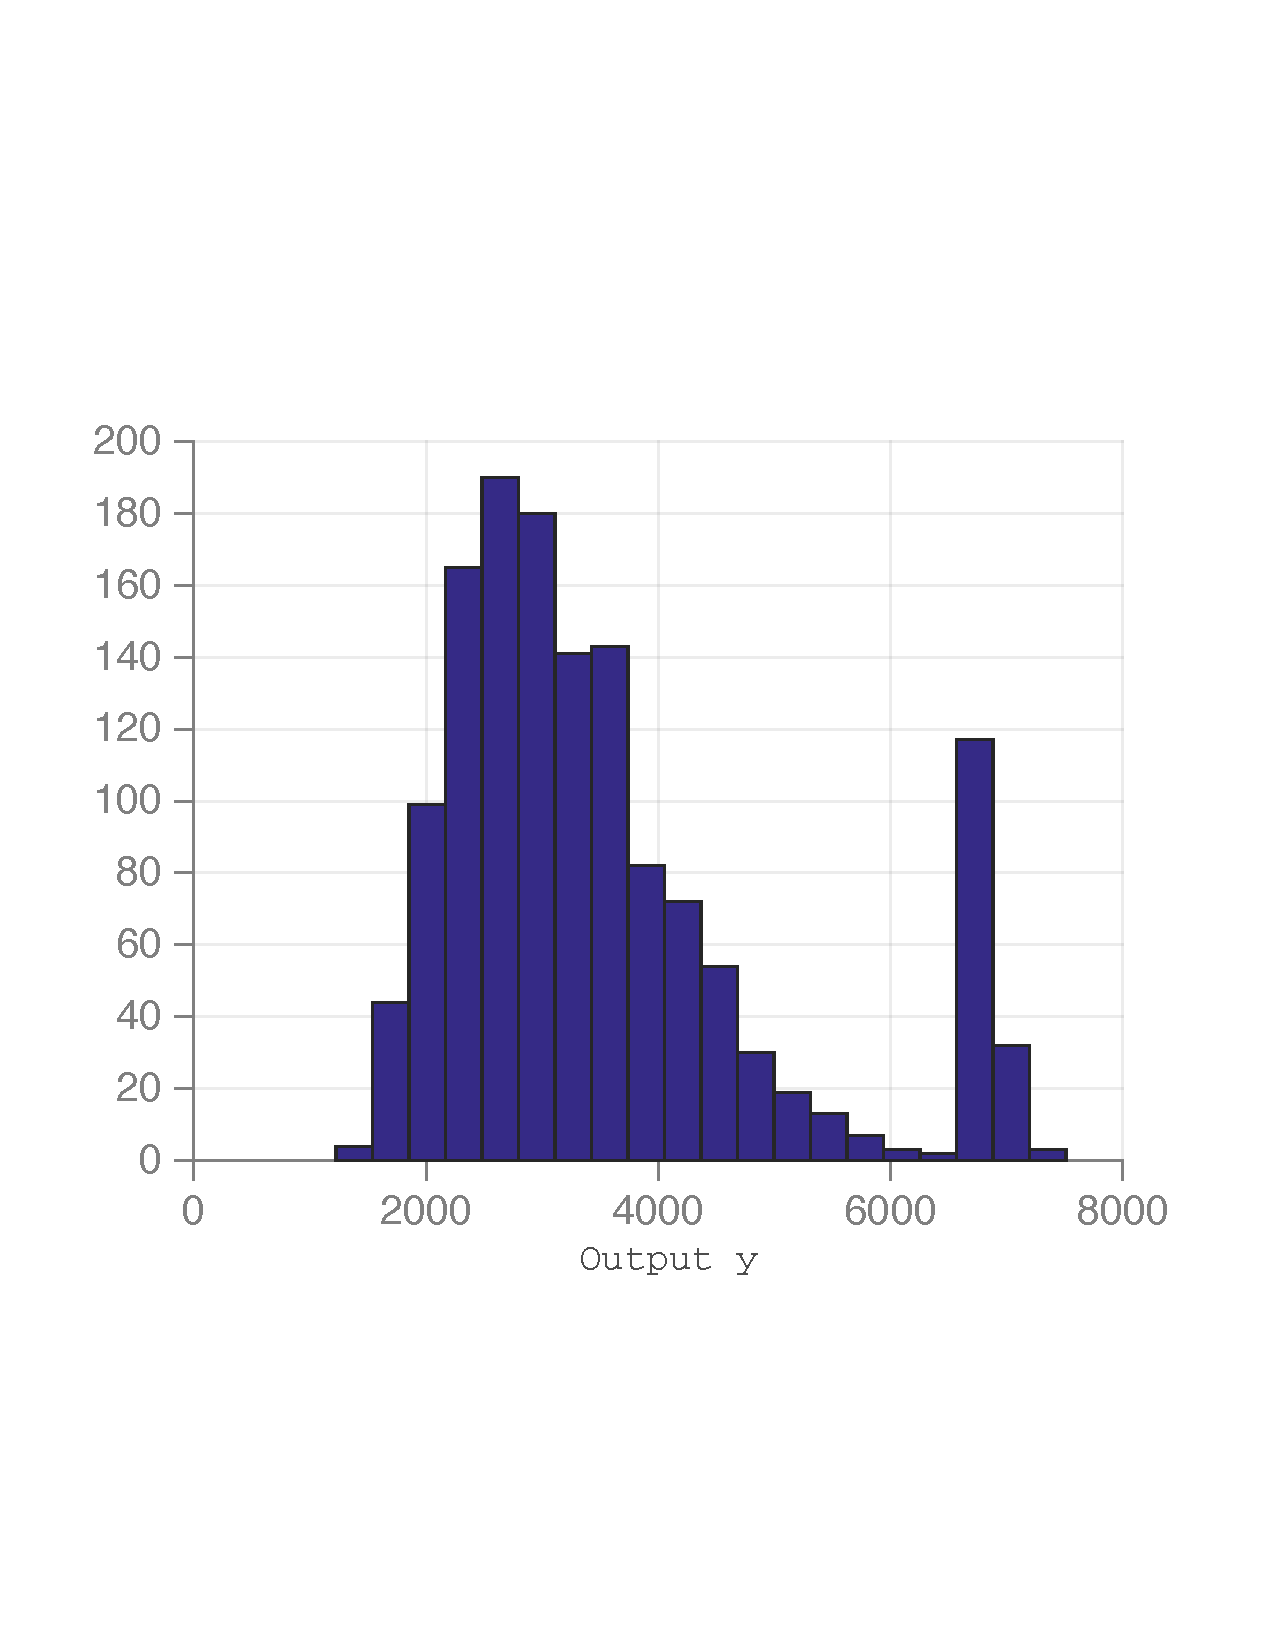
\includegraphics[width=2.5in]{figures/regression/hist-Y.pdf}
      \label{fig:histY}
    }
    \hfill
    \subfigure[$X_{35}$ seems to enable us to linearly separate the two models simply]{
      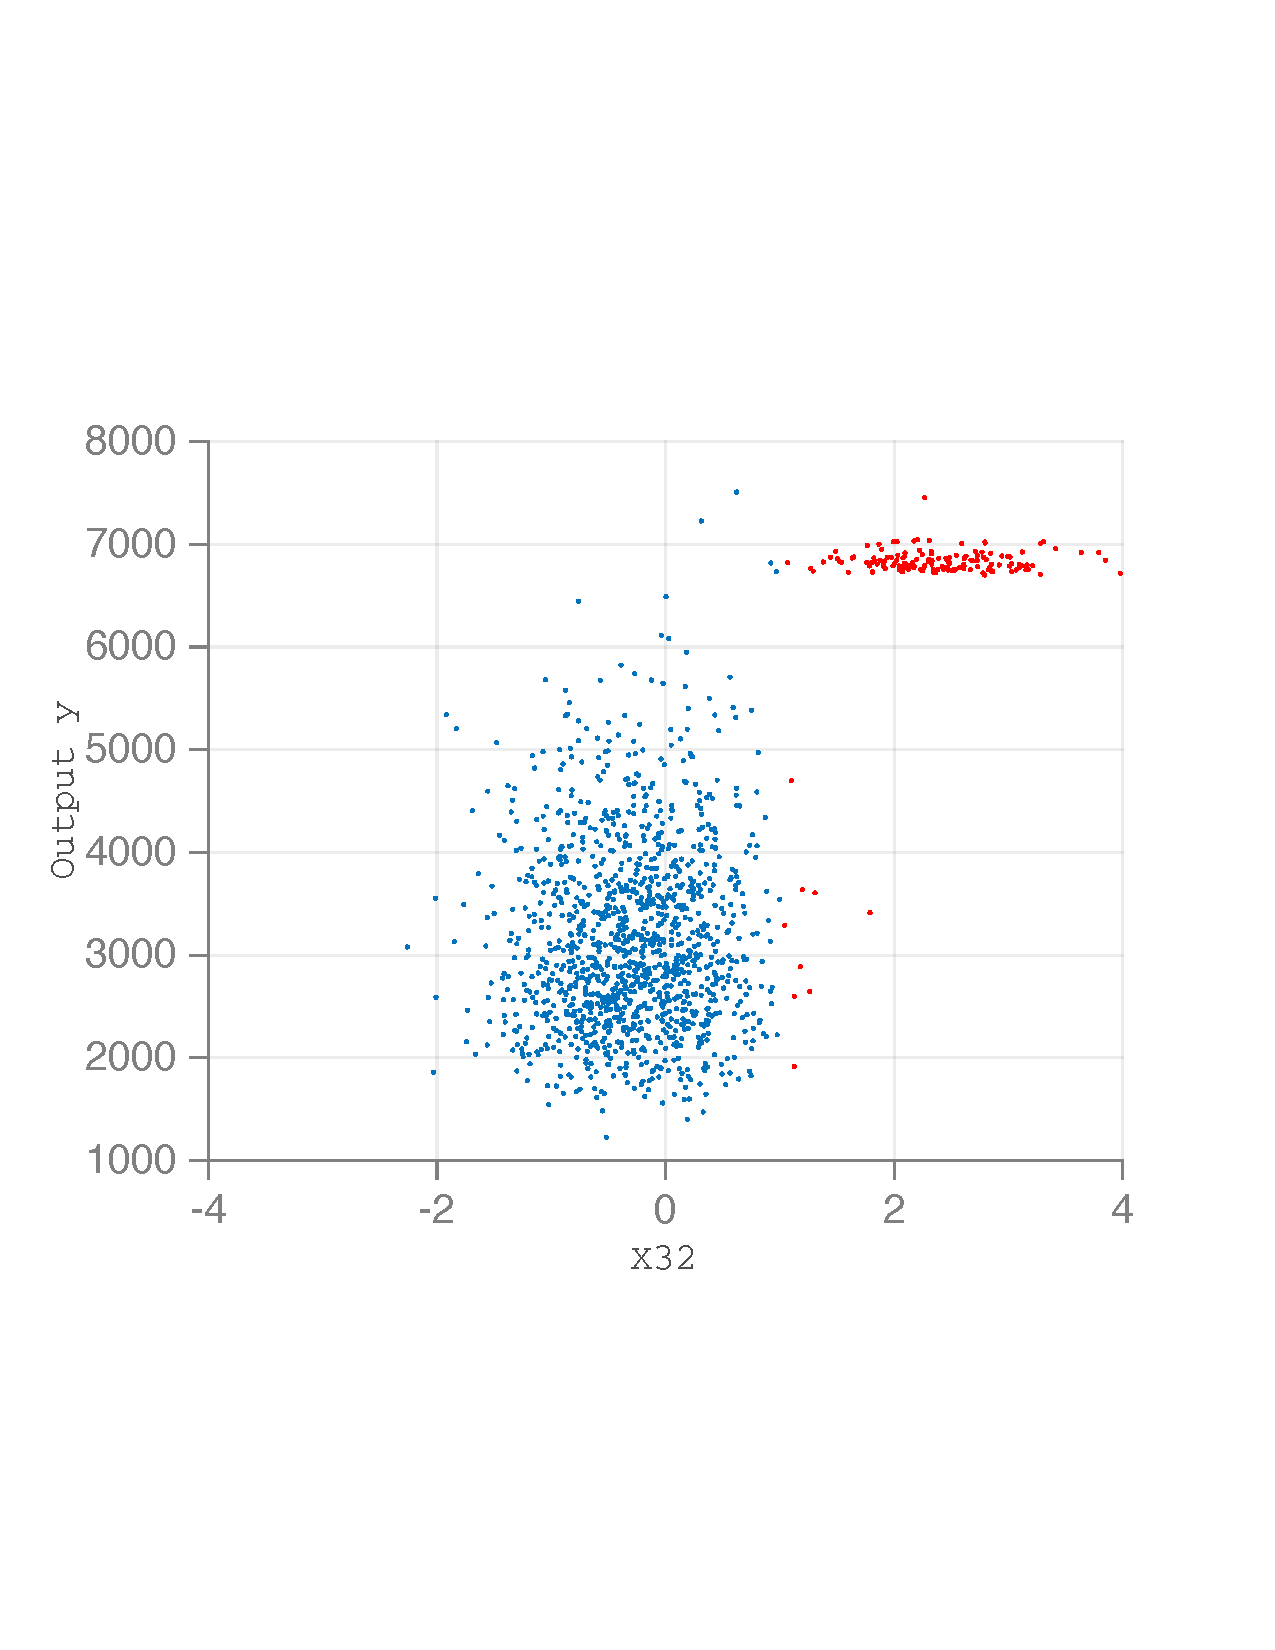
\includegraphics[width=2.5in]{figures/regression/model-separation-X35.pdf}
      \label{fig:twoModelsX35}
    }
    \hfill
    \subfigure[First try at separating the two models on regression data using $X_{35} > 1$]{
      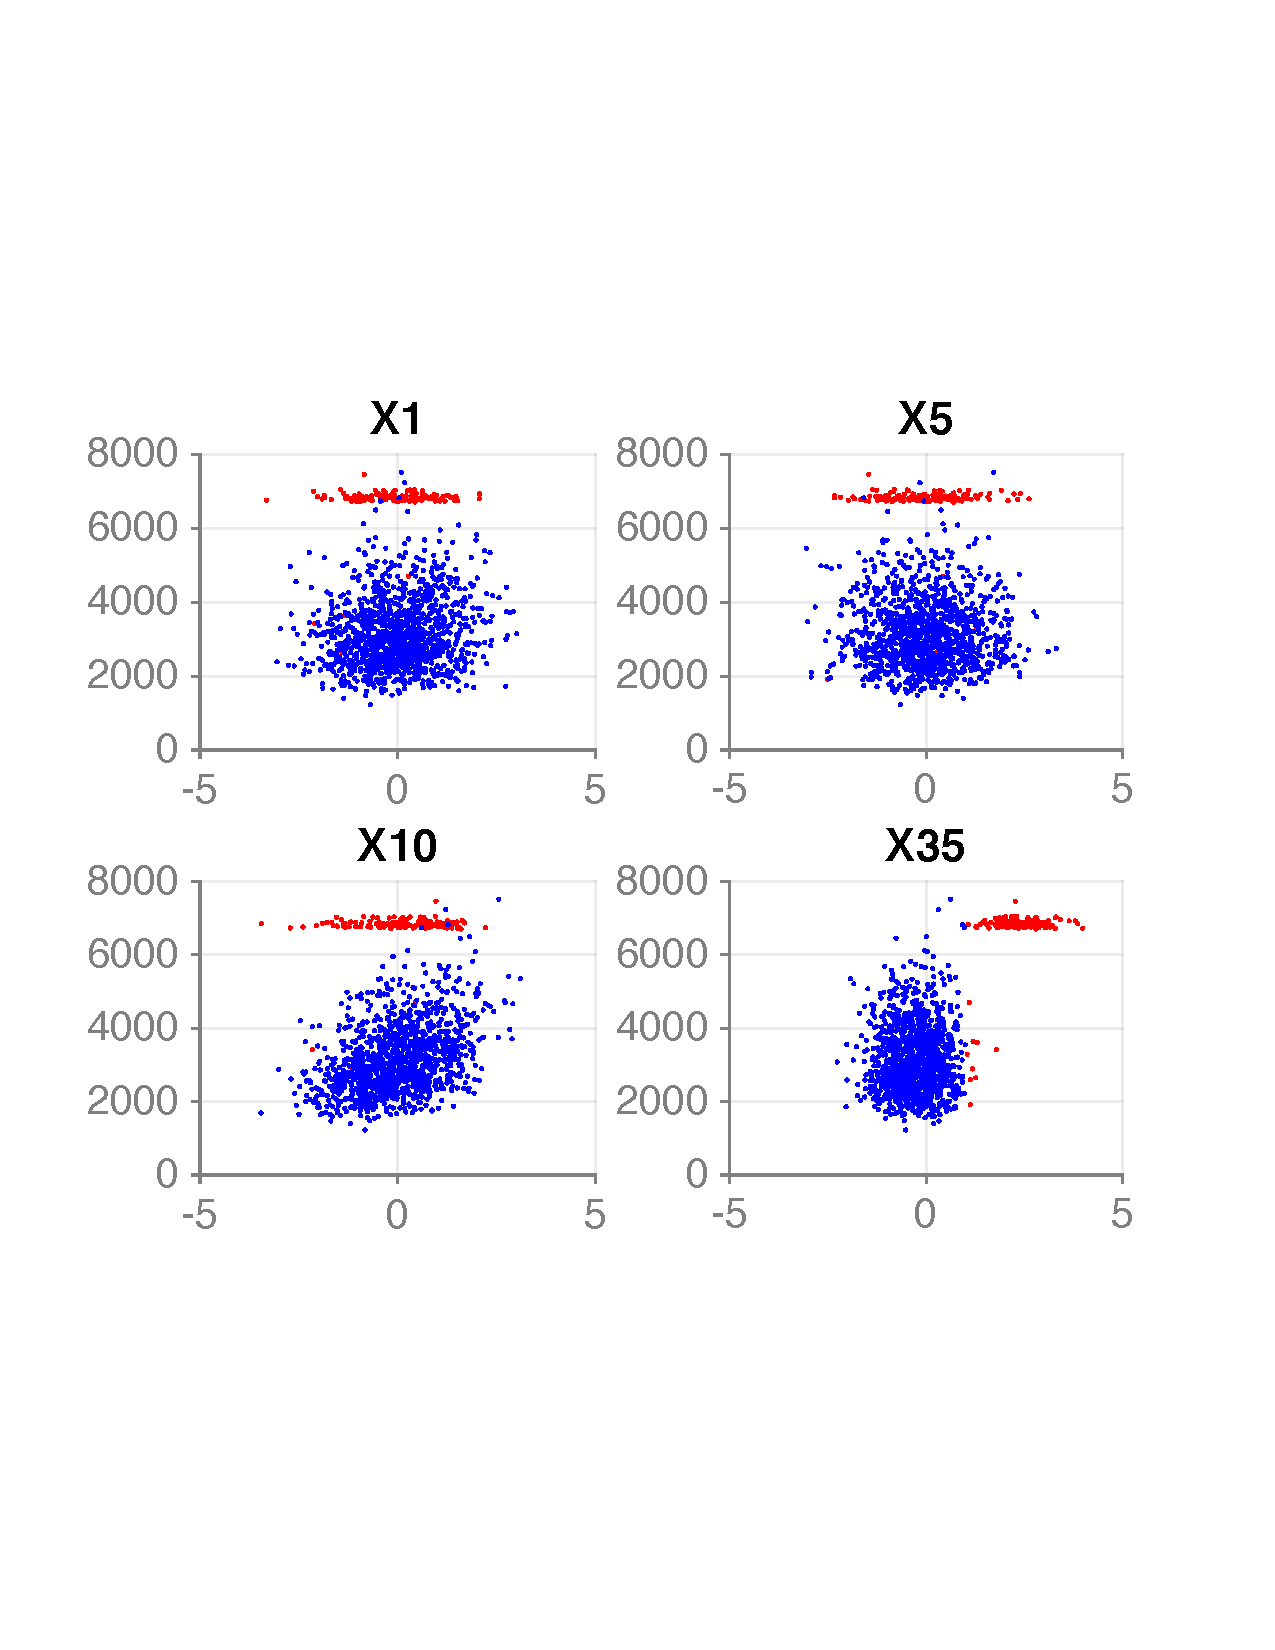
\includegraphics[width=4in]{figures/regression/model-separation-rough.pdf}
      \label{fig:twoModelsRough}
    }
    \caption{}
  \end{figure}

  \subsection{Model separation}
  From our explorative data analysis phase, we emitted the hypothesis that our dataset could be represented by two distinct models. We checked our intuition by learning a single model on the whole dataset, and compared it with a two-model fit learnt over a roughly split dataset. The test error decreased dramatically when using two models. This motivated us to learn a classifier in order to refine the dataset split.

  We chose a threshold on the output value ($y_n > 6200$) and used it to convert $\mathbf{y}$ to a $\{0, 1\}$ label vector. This enabled us to apply logistic regression directly and learn a classifier. We checked the result visually by plotting the two parts of the dataset in different colors.

  The first model, denoted $M_1$, is not trivial. On the other hand, the second model, $M_2$, can be described simply with a (high) constant output value.

  \subsection{Feature transformations}
  In order to describe $M_1$ accurately, we investigated potential feature transformations which would increase the power of expression of our model. We needed to strike a balance between underfitting (purely linear model) and overfitting (high-degree polynomial transformation). To select the degree of polynomial basis expansion, we developed a script which, for each degree:
  \begin{itemize}
    \item Applies polynomial basis expansion up to degree $d$
    \item Creates a large number $s$ of trials (test / train splits), enabling us to validate the stability of our results
    \item For each trial, applies ridge regression, which selects the best $\lambda$ penalization parameter using grid search over a logarithmic range of candidate values.
  \end{itemize}

  Note that we are using ridge regression in this script. Indeed, the polynomial basis expansion makes the extended input matrix rank deficient. Least squares is therefore not suitable.

  We could then plot the repartition of test and train error over the $s$ trials, allowing us to select the most adapted degree with high confidence about the stability. Figure \ref{fig:basisExpansionTestError} illustrates clearly the biais / variance tradeoff. As the degree increases, our model is able to fit the training data better. Since we are using a regularization parameter, test error decreases as well until a certain point, but becomes the predictor become unable to generalize from a certain point. In this case, polyomial extension of degree 4 provides the best expected test error.

  \begin{figure}[h]
    \center
    \subfigure{
      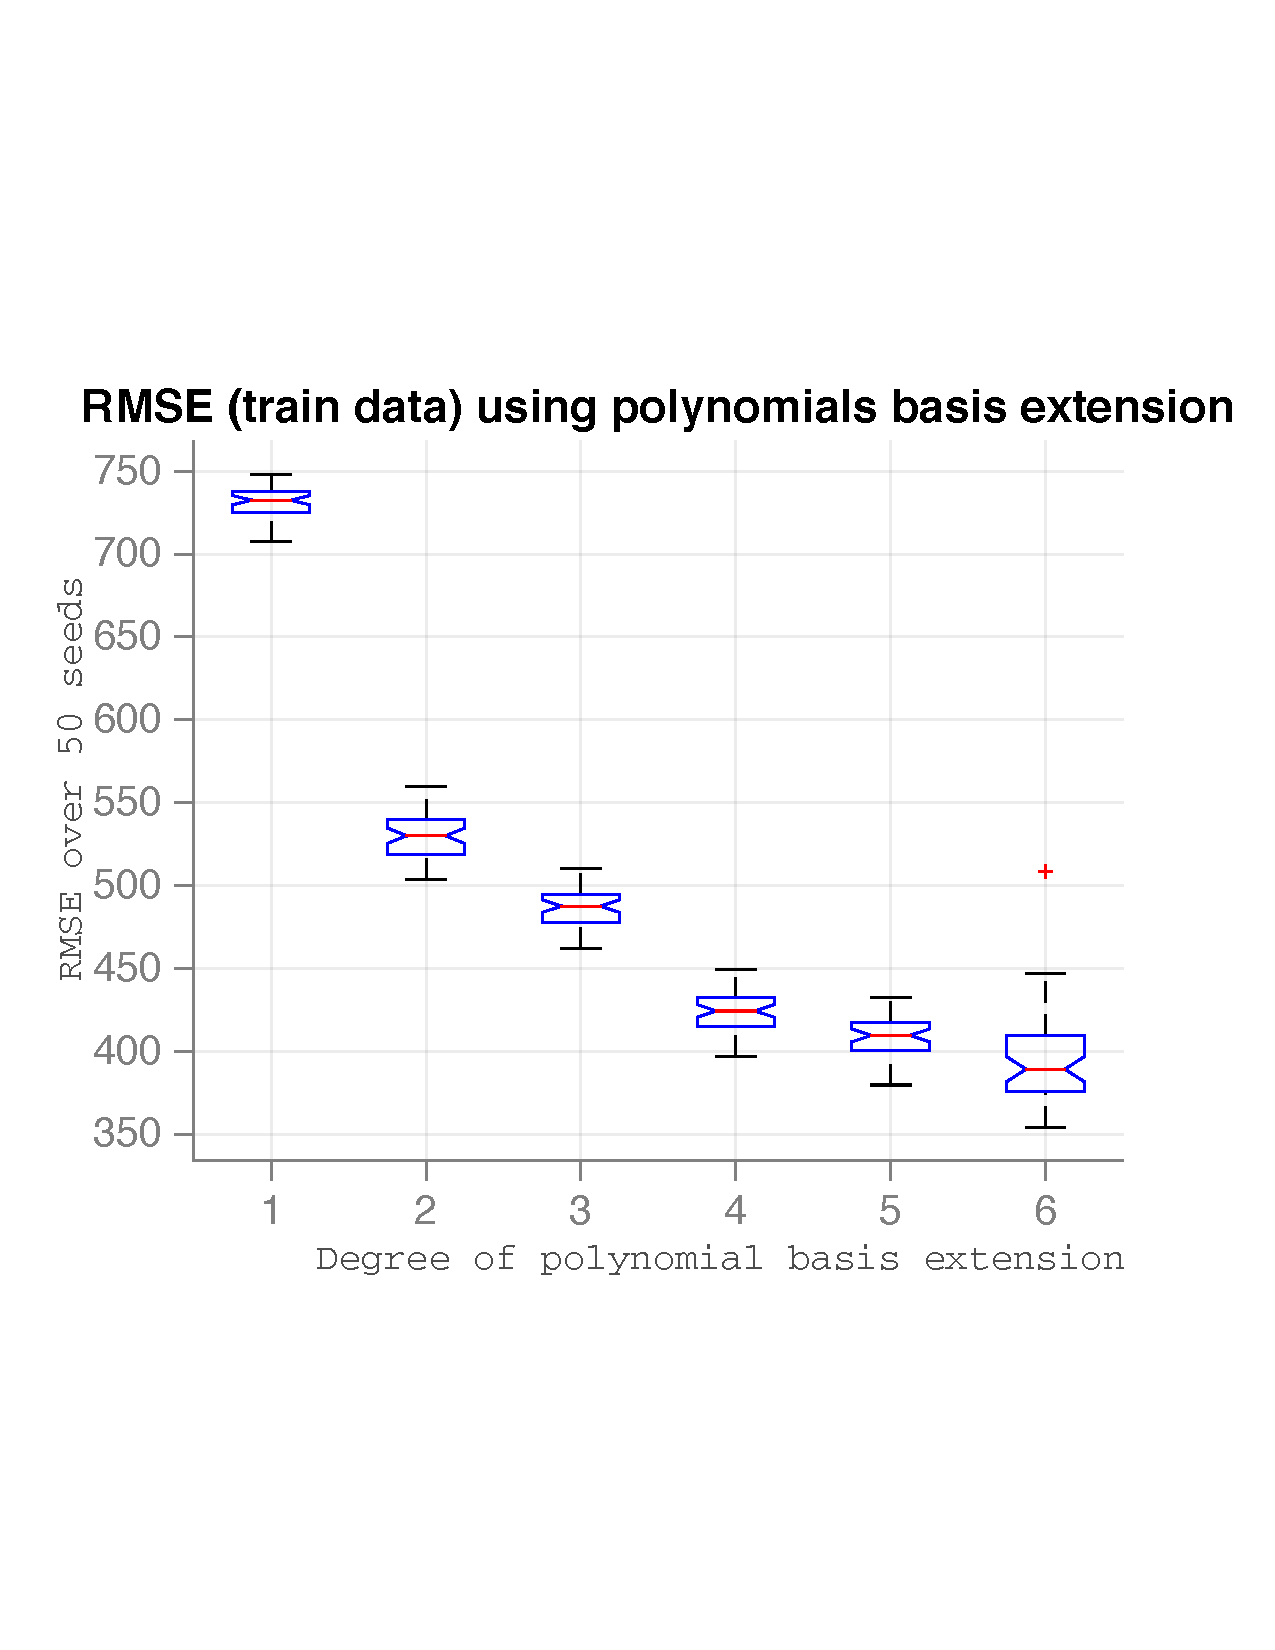
\includegraphics[width=2.5in]{figures/regression/basis-extension-train-error.pdf}
    }
    \hfill
    \subfigure{
      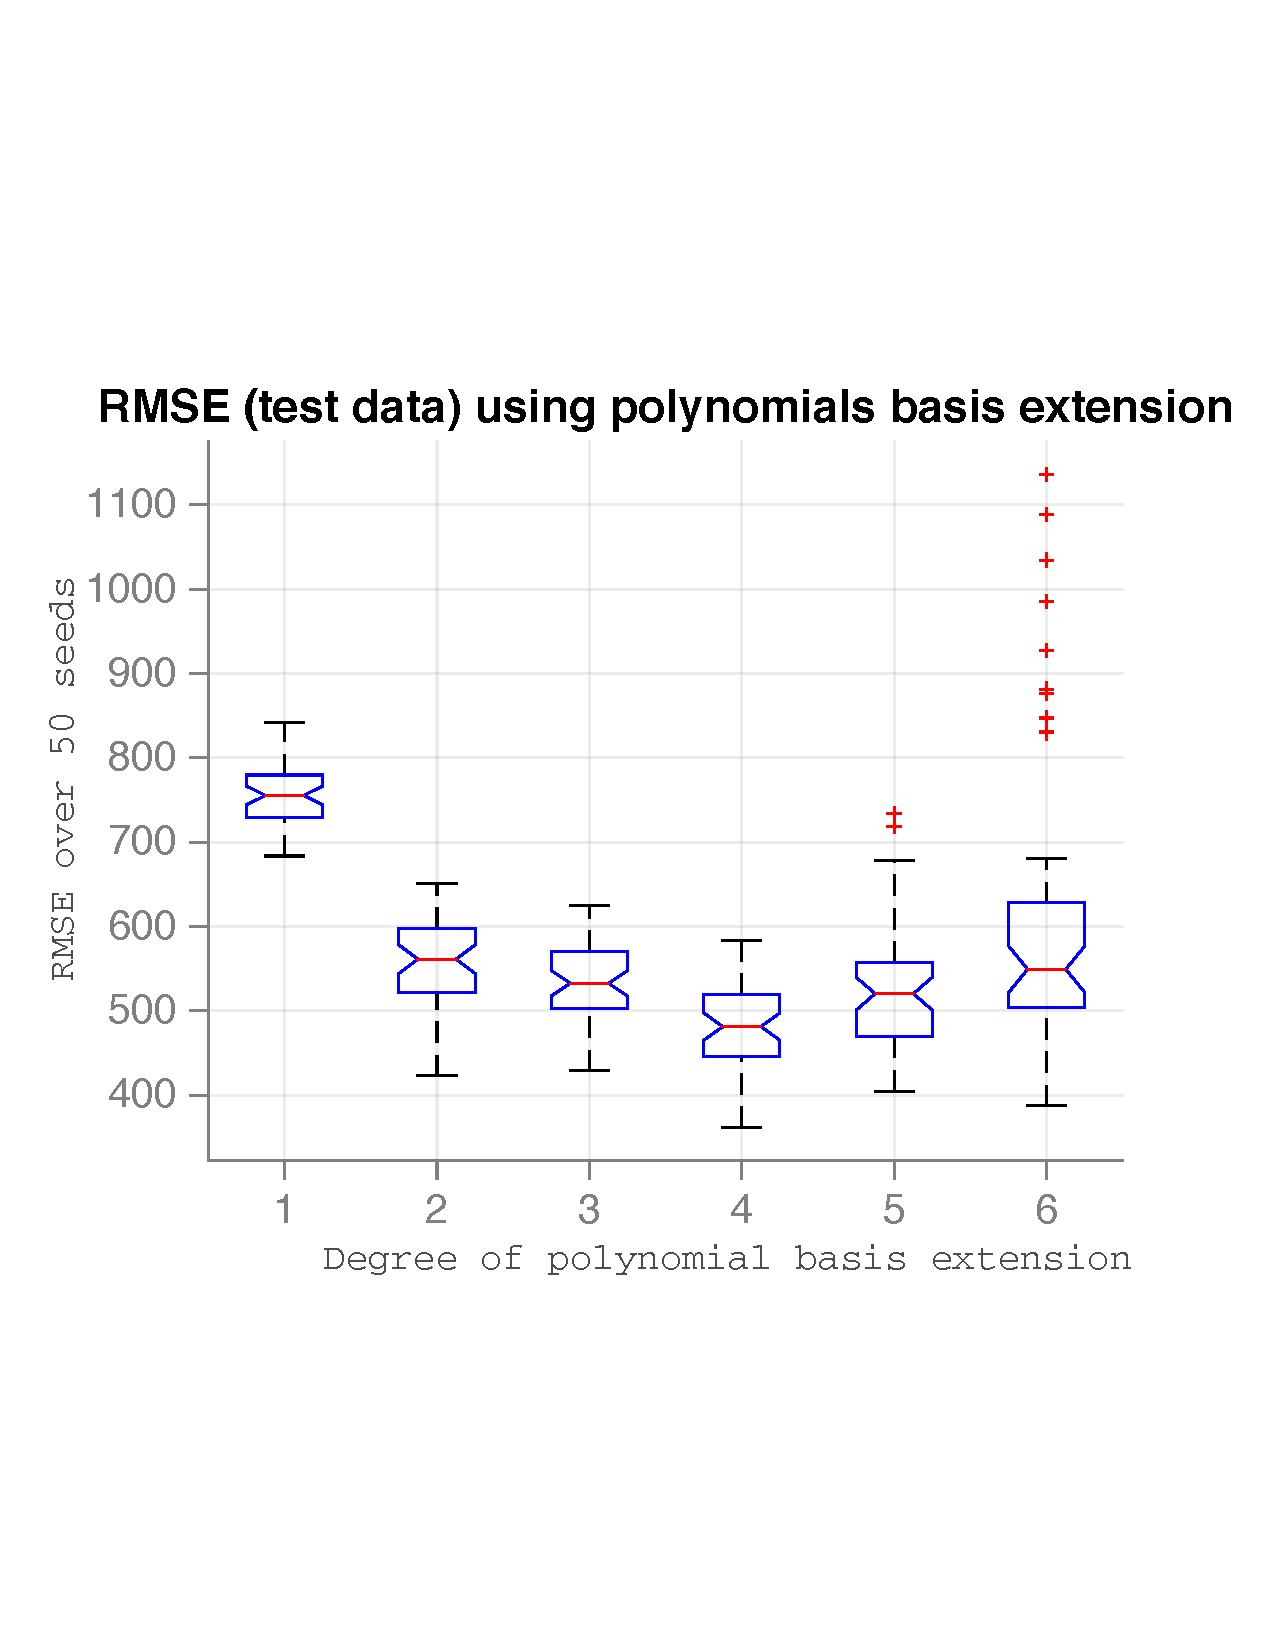
\includegraphics[width=2.5in]{figures/regression/basis-extension-test-error.pdf}
    }
    \caption{Our model selection procedure illustrates the biais / variance tradeoff}
    \label{fig:basisExpansionTestError}
  \end{figure}

  We thus chose to apply polynomial expansion of degree 4 to our subset of inputs $X_{M_1}$. We were careful not to transform the binary variables. We obtain dimensionality $D_{M_1} = 156$ and the risk to overfit, which is why we applied ridge regression next to learn our model parameters.

  Note that our implementation of ridge regression selects the regularization parameter $\lambda$ automatically by computing the expected test error using k-fold cross validation (kCV). For this dataset, we used $k = 10$ and $\lambda$ to be selected among a logarithmic range of 100 values from $1$ to $10^2$.

  \subsection{Regression fit and prediction} \label{regression-fit}
  With the necessary data analysis and pre-processing taken care of, we were able to easily learn the parameters for our two models:
  \begin{itemize}
    \item $M_1$: model parameter vector $\beta$ is learnt using ridge regression with automatic $\lambda$ selection. The algorithm selected $\lambda \approx 50$.
    \item $M_2$: a constant output value equal to the mean of the outputs from the training observations. We were careful to remove obvious outliers.
  \end{itemize}

  We were finally able to produce our \textbf{hybrid} predictor, which successively:
  \begin{enumerate}
    \item Classifies any new input using our learnt classifier.
    \item If the input follows $M_2$, outputs the learnt constant value.
    \item Otherwise, applies dummy encoding, basis expansion and outputs the prediction corresponding to model $M_1$ using our learnt parameter $\beta$.
  \end{enumerate}

  We verified the performance of our final predictor by computing its RMSE error and comparing it with simpler predictors using 10-fold cross validation. The average RMSE are summarized in Table \ref{predictorValidation}.

  From this comparison table, we can notice that ridge regression does not bring a significant improvement compared to least squares if no feature transformation is performed. This is expected. However using a polynomial expansion of degree 4 and then applying ridge regression decreases considerably the test error. This is coherent as well, since the regularization parameter prevents overfitting. Our hybrid predictor combining two models gives us the lowest expected train error.

  \begin{table}[h]
    \center
    \begin{tabular}{|r|c|c|}
      \hline
      \textbf{10-fold cross validation estimates} & Train RMSE & Test RMSE \\
      \hline
      Constant output                             & 0.999596   & 0.998914  \\
      \hline
      Least squares                               & 0.512271   & 0.534063  \\
      \hline
      Ridge regression                            & 0.513674   & 0.532057  \\
      \hline
      Basis expansion and ridge regression        & 0.298089   & 0.335880  \\
      \hline
      Hybrid predictor                            & 0.168528   & 0.203762  \\
      \hline
    \end{tabular}
    \caption{Validation of our prediction by comparison with simpler models using cross-validation}
    \label{predictorValidation}
  \end{table}

  Finally, we produced our predictions for the given \texttt{X\_test} input vector using the hybrid predictor and wrote them to \texttt{predictions\_regression.csv}.

\section{The classification dataset (D2)}
  Much of the intuition and techniques gained from D1 carried over directly to D2. We report the most interesting results below.

  \subsection{Dataset description}
  This dataset has $N = 1500$ data examples with dimensionality $D = 32$, as well as $N' = 1500$ test examples. Out of these 32 features, 29 are real-valued and 3 are categorical.\\
  Output $\mathbf{y}$ is a binary variable, which implies that we are faced with a classification problem. 448 examples belong to class $C_1$ (for which $y = 0$) and 1052 examples belong to $C_2$. Like before, our goal is to produce predictions for test examples, as well as an approximation of the test error.

  \subsection{Data visualization and cleaning}
  We performed data analysis steps similar to the one taken for D1. However, spotting outliers visually on a classification dataset is not an easy task, therefore we have assumed that a data point is an outlier if for any feature it lies more than 10 standard deviations away from the median. We obtained a ``clean'' dataset of 1469 examples.

  For more convenience of manipulation, we moved categorical variables to the last columns of the input matrix and used dummy encoding for each of them. This gives us a total of 46 input variables.

  \subsection{Feature transformations}
  Applying feature transformations to D2 proved hard than it was for D1. Rank deficiency appeared systematically and the prediction results were not generalizing well, even though we used a regularization term. We found empirically that it improved the results to append the squareroot of the real-valued features to the input matrix. Since this transformation did not prevent generalization nor caused rank deficiency, we used it in the following steps.

  \subsection{Logistic regression fit}
  In order to quickly get a baseline for the quality of our models, we learnt two of the simplest models: constant-valued and using least-squares. We carried on by applying logistic regression and saw a dramatic improvement in the expected quality of the results (from $30\%$ of misclassifications to less than $10\%$). We made sure to use the ``log-exp'' trick (seen during the exercise sessions) to avoid numerical issues.

  Finally, we applied penalized logistic regression to obtain our best result over D2. As explained in section \ref{regression-fit} for ridge regression, our penalized logistic regression function selects the most appropriate regularization parameter $\lambda$ among a range of values by computing the expected test error. In this case, $\lambda \in [10^{-2}; 10^2]$.

  \subsection{Predictions}
  After validating the stability of our results with 10-fold cross validation, we used all available data examples to train a model using penalized logistic regression. We generated the classification probabilities corresponding the \texttt{X\_test} input vector and wrote them to \texttt{predictions\_classification.csv}.

  We check our output visually on Figure \ref{fig:classification-output} and verify that the results are in $[0; 1]$. We observe a distribution skewed towards 1, which is consistant with the fact that about $70\%$ of the training examples belong to $C_2$.

  \begin{figure}[h]
    \center
    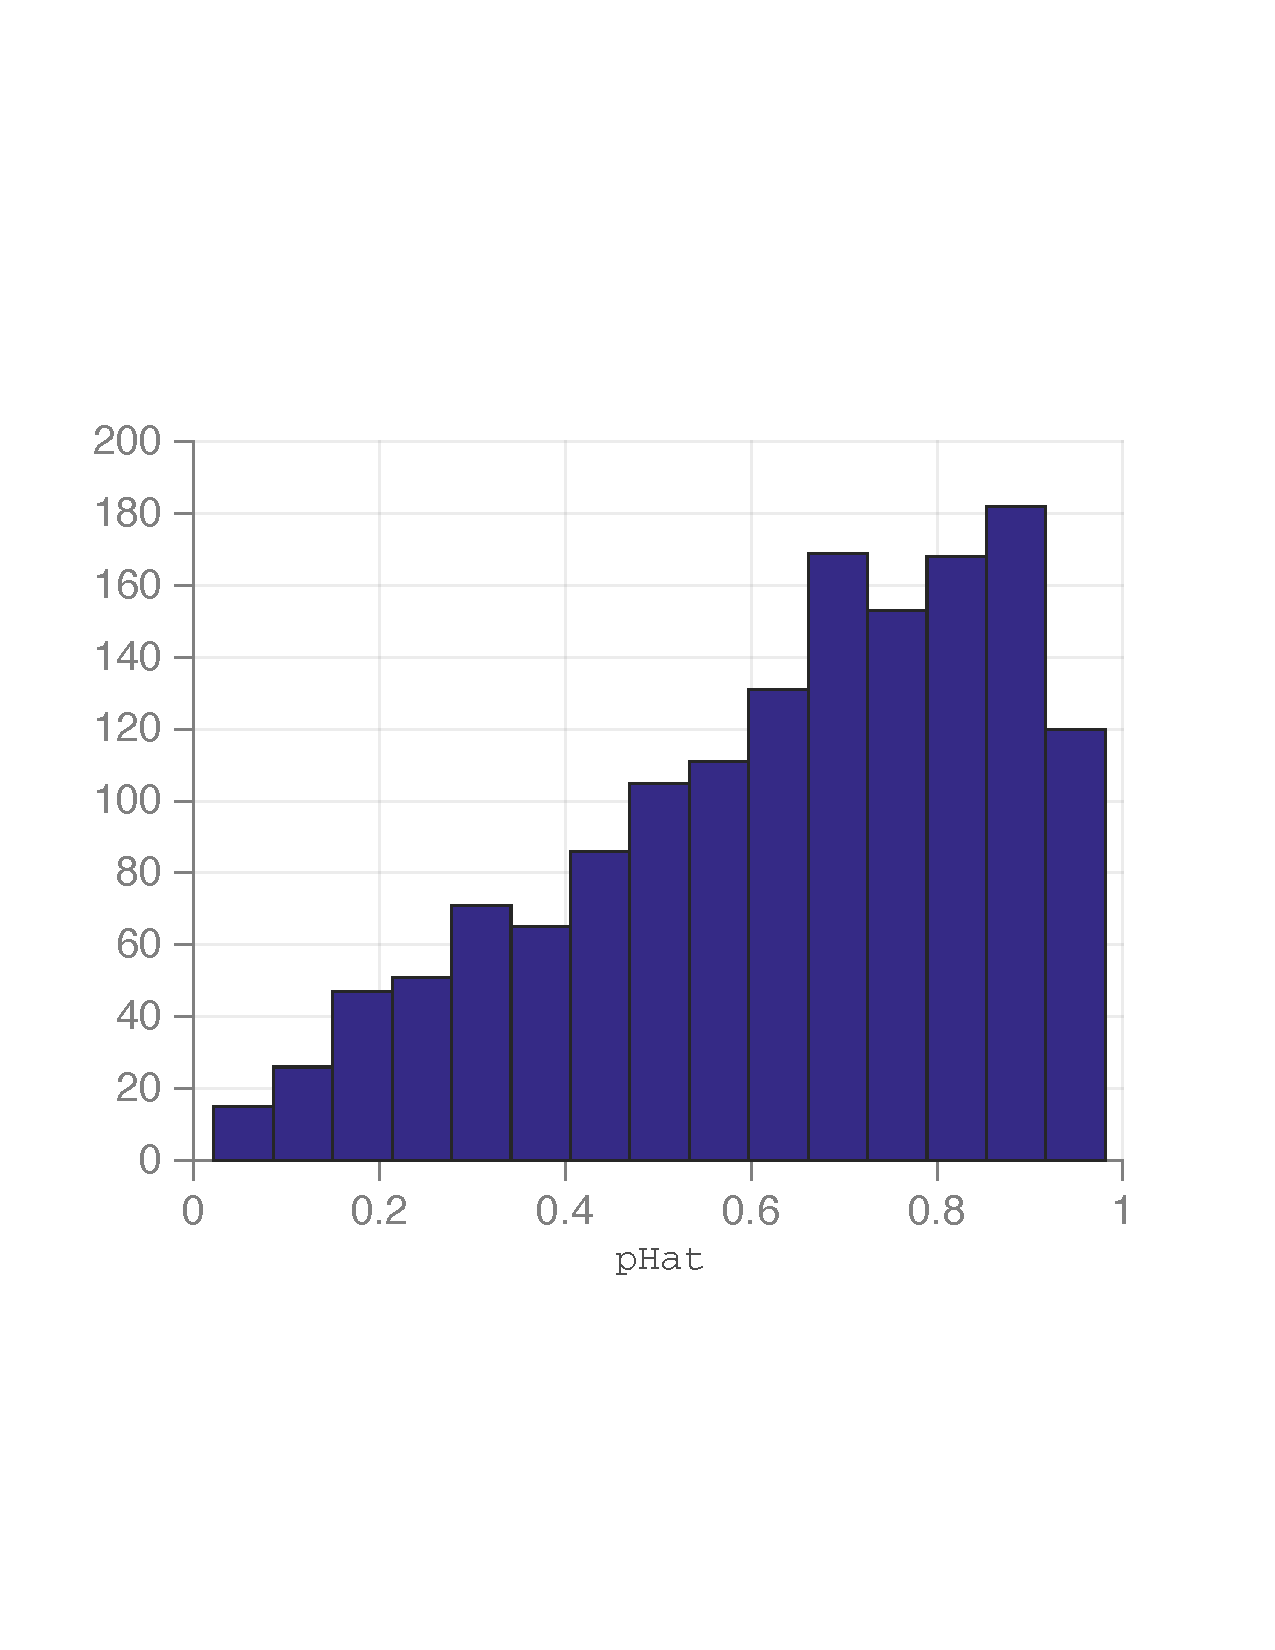
\includegraphics[width=2.5in]{figures/classification/output-phat.pdf}
    \caption{Repartition of the output probabilities}
    \label{fig:classification-output}
  \end{figure}

\section{Summary}
In this report, we analyzed 2 datasets: one regression dataset and one classification dataset. 

In our regression dataset we found that our data was following 2 models. For the most complex model we found ridge regression applied after features transformations with a polynomial function of degree 4 is a reasonable fit. On the simplest model, a constant value returns a good fit. We estimate that the average test error is TODO

In our classification dataset, we had to do binary classification. We found that... We estimate the average test error is TODO

\subsubsection*{Acknowledgments}
  We would like to thank Prof. Emtiyaz Khan and the teaching assistants for creating this project. It was a great opportunity for us to put in practice our the Machine Learning techniques seen in class on a serious dataset. We also would like to thank them for their availability throughout the semester.\\
  Most ML functions and algorithms were based on the lecture notes or code examples provided by the teaching team for the exercise sessions. We developed several exploratory and application scripts to make use of these techniques. Several helper functions were provided by Prof. Emtiyaz Khan (CSV output, plot prettifying and output, etc).

\subsubsection*{References}
  During implementation, we referred to the lecture and exercise instructions provided by Prof. Emtiyaz Khan and the teaching team. Moreover, we found Andrew Ng's MOOC on Coursera to be helpful, since a few short videos covered precisely points which we were unsure about.

\end{document}
